\documentclass[11pt]{article}
\usepackage{mathtools}
\usepackage{mdframed}
\usepackage{fullpage}
\usepackage{amsfonts}
\usepackage{tikz}
\usepackage{fancyhdr}
\usepackage{graphicx}
\usepackage{lastpage}


%edit this for each class
\newcommand\name{John Collin Vincent}
\newcommand\classname{}
\newcommand\assignment{}


\newcounter{excounter}
\setcounter{excounter}{1}
\newcommand\ques[2]{\vskip 1em  \noindent\textbf{\arabic{excounter}\addtocounter{excounter}{1}.} \emph{#1} \noindent#2}
\newenvironment{question}{\ques{}\begin{quote}}{\end{quote}}
\newenvironment{subquestion}[1]{#1) \begin{quote}}{\end{quote}}

\pagestyle{fancy}
\rfoot{\name, page \thepage/\pageref{LastPage}}
\cfoot{}
\rhead{}
\lhead{}
\renewcommand{\headrulewidth}{0pt}
\renewcommand{\footrulewidth}{0pt}
\DeclarePairedDelimiter\ceil{\lceil}{\rceil}
\DeclarePairedDelimiter\floor{\lfloor}{\rfloor}


\begin{document}


  {\bf \classname \hspace{1cm} \assignment\hfill \name}
  \vskip 2em


  \begin{question}
    \begin{subquestion}{a}
        the loop will never check the 0\textsuperscript{th} index. the solution would be to change
        the loop exit condition to $i \le 1$
    \end{subquestion}
    \begin{subquestion}{b}
        if the array is null then the function will throw a null pointer at the x.length-1 section of the for loop and never execute the faulty line
        of $i > 0$
    \end{subquestion}
    \begin{subquestion}{c}
        if you use the array ${1,2,3}$ an use the $y=3$ then the fault will be executed but i will never get to 0 so the program never enters
        an error state.
    \end{subquestion}
    \begin{subquestion}{d}
        if you use the array ${1,2,3}$ an use the $y=4$ then the program will enter an error state since it will skip over checking the
        element $1$ but it will still return the correct result. So there will not be a failure.
    \end{subquestion}
    \begin{subquestion}{e}
        The first error state is when the loop hits the line $i>0$ when $i = 0$. this causes the program to exit the loop before checking the index
        that contains the value that you are looking for.
    \end{subquestion}
    \clearpage
    \begin{subquestion}{f}
        \hspace*{-4.2cm}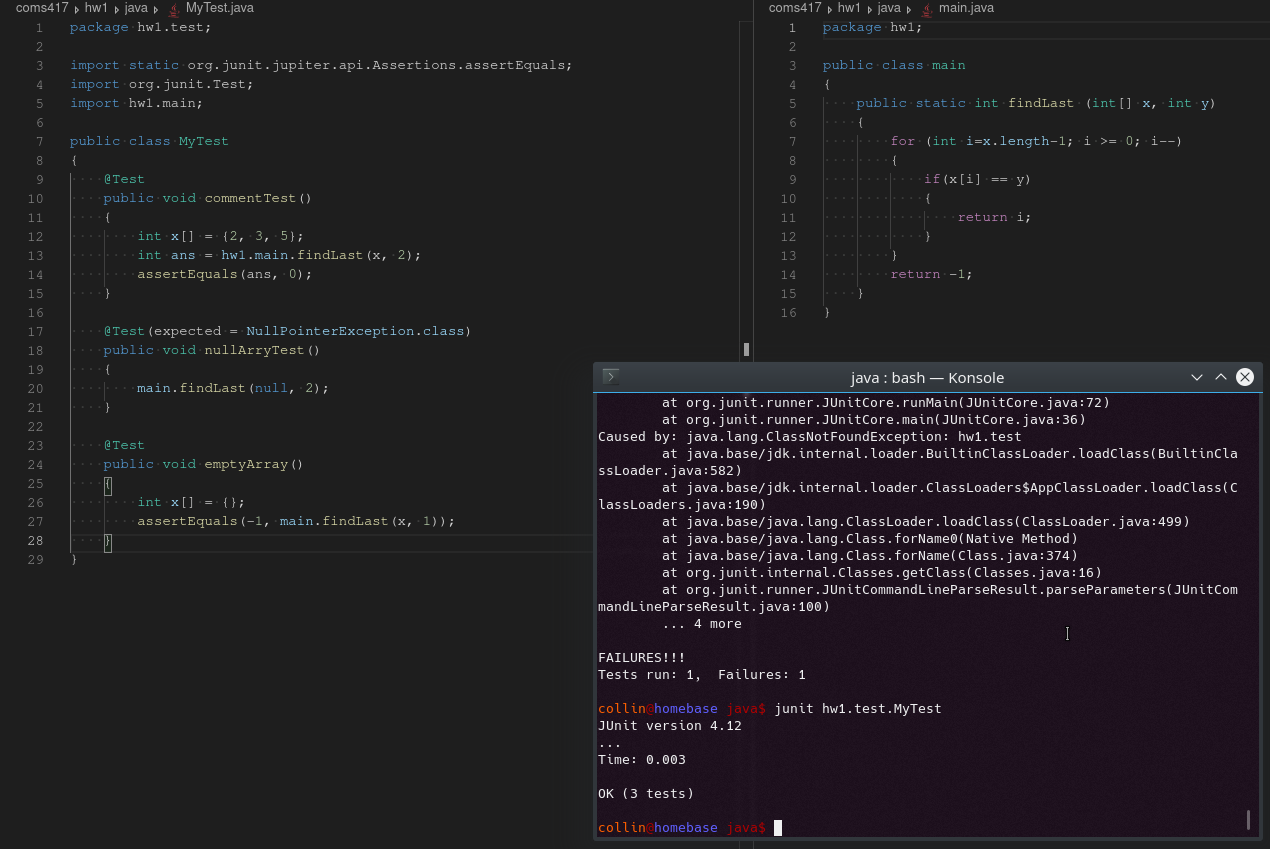
\includegraphics[width=1.3\textwidth]{coms417/hw1/question1.png}
    \end{subquestion}
  \end{question}

    \clearpage

    \begin{question}
        \begin{subquestion}{a}
            The issue is that the super clone method really returns a Vehicle so there will be a class cast exception
            for every class to trucks clone method. The solution would be to utilize the Object clone method
            in truck to preserve the dynamic type of any subclass.
        \end{subquestion}
        \begin{subquestion}{b}
            Any test that doesn't run the Trucks clone method will not execute the fault.
        \end{subquestion}
        \begin{subquestion}{c}
            This is not possible because every execution of the Trucks clone will result in an error state.
        \end{subquestion}
        \begin{subquestion}{d}
            This is not possible because it is not expected that the clone throws a ClassCastException in any scenario,
            however it always will.
        \end{subquestion}
        \begin{subquestion}{e}
            The first error state is during the second line in the truck clone where it does ((Truck) result)
        \end{subquestion}
        \clearpage
        \begin{subquestion}{f}
            here i have the vehicle class, i made the truck class a public static class of vehicle to
            make things easier on myself but the behavior is the same. you can see the changes i made to the
            vehicle clone method. Since they didn't declare that the clone would throw any exceptions I
            decided to just catch the exception from the Object clone method.\\
            \hspace*{-4.2cm}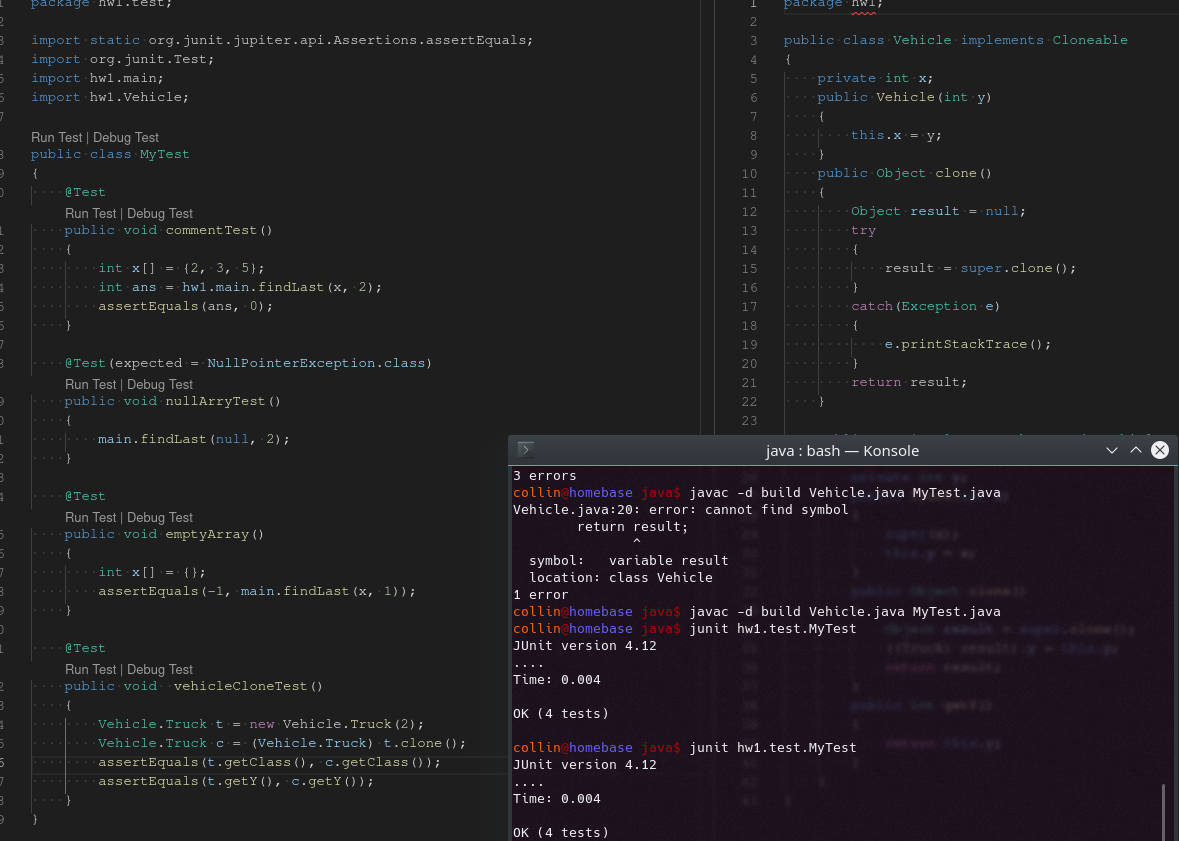
\includegraphics[width=1.3\textwidth]{coms417/hw1/question2.png}
        \end{subquestion}
    \end{question}

    \clearpage

    \begin{question}
        \begin{subquestion}{a}
            A test that calls computePrimes with $n=1$ will never reach the fault, because the isPrime boolean is
            never true when it reaches the if statement containing the fault.
        \end{subquestion}
        \begin{subquestion}{b}
            A test that calls computePrimes with $n<=8$ will reach the fault because 2 and 3 are prime but
            it will not infect because it never reaches a number that ends in 9.
        \end{subquestion}
        \begin{subquestion}{c}
            A test that calls computePrimes with a large number will infect the state but as long as they don't make
            any calls that interact with the later primes, like only calling getFirstPrime and checking it is 2, the
            fault won't propagate.
        \end{subquestion}
        \begin{subquestion}{d}
            A test that calls computePrimes with a large number, then iterates the list and makes sure all the values are prime.
            This will not reveal the fault because all the values are truly prime and there is no verification that all the primes are there.
        \end{subquestion}
        \begin{subquestion}{e}
            A test that calls computePrimes with a large number then uses a string that matches the output of toString will manually
            calculated primes up to the number used will reveal the fault.
        \end{subquestion}
    \end{question}


\end{document}
